\begin{lstlisting}
•    Section 4.2:  17, 18, 19, 23, 25,  27(a)(c)  
•    Section 4.4:  6(a), 7,  9,  26,  30,  31    
\end{lstlisting}
\begin{exercise}
\begin{figure}[H]
\centering
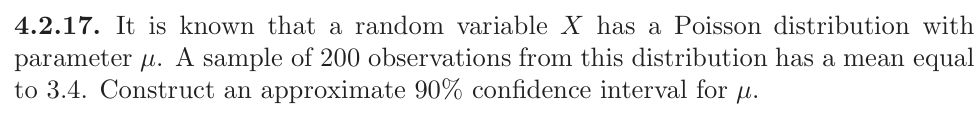
\includegraphics[width=\textwidth]{1-hw5-2025032722.png}
% \caption{}
\label{}
\end{figure}
\end{exercise}
The statistic model is
\[
\mathfrak{F}=\left\{  f(n;\mu)=\frac{\mu^{n}}{n!}e^{ -\mu }:n\in \mathbb{N},\mu>0  \right\}
\]
Let  $X_1,\dots,X_n$ are random sample of distribution $\text{Poi}(\mu)$. To calculate the mle of $\mu$,
\[
l(\mu)=\sum_{k=1}^{n} \log\left( \frac{\mu^{x_k}}{x_k!}e^{ -\mu } \right)=\sum_{k=1}^{n} (-\mu+x_k\log \mu-\log(x_k!))=-n\mu+\sum_{k=1}^{n} x_k\log \mu-\sum_{k=1}^{n} \log(x_k!)
\]
Then
\[
\frac{ \partial l(\mu) }{ \partial \mu } =-n+\frac{1}{\mu}\sum_{k=1}^{n} x_k
\]
Thus the mle of $\mu$ is
\[
\widehat{\mu}_n=\frac{1}{n}\sum_{k=1}^{n} X_k
\]
Thus $\widehat{\mu}_n\sim\text{Poi}(\mu)$. $\mathbb{E}\widehat{\mu}_n=\mu,\mathrm{Var}\widehat{\mu}_n=\mu$. When $n$ is large,
\[
\widehat{\mu}_n\overset{ \mathcal{D} }{ \to } N\left( \mu,\frac{\mu}{n} \right)\implies\frac{\widehat{\mu}_n-\mu}{\sqrt{ \mu/n  }}\overset{ \mathcal{D} }{ \to } N(0,1)
\]
Let $z_{\alpha/2 }\coloneqq \Phi ^{-1}(1-\alpha/2 )$ where $\Phi$ is the standard normal distribution. Then the $1-\alpha$ confidence interval of $\mu$ is (we replace $\mu/n$ by its estimator $\widehat{\mu}_n/n$)
\[
C_n=\left( \widehat{\mu}_n-z_{\alpha/2 }\sqrt{ \frac{\widehat{\mu}_{n}}{n} },\widehat{\mu}_n+z_{\alpha/2 }\sqrt{ \frac{\widehat{\mu}_n}{n} } \right)
\]
Put $n=200,\widehat{\mu}_n=3.4,\alpha=0.1$ then
\[
C_n=(3.19,3.61)
\]
\begin{exercise}
\begin{figure}[H]
\centering
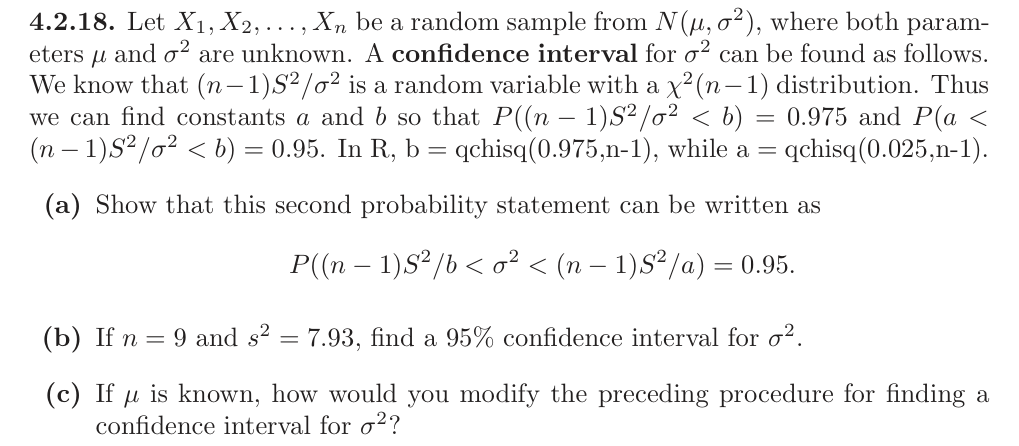
\includegraphics[width=\textwidth]{2-hw5-2025032722.png}
% \caption{}
\label{}
\end{figure}
\end{exercise}
(a) Trivial.

(b) $a=2.180,b=17.535$.
\[
C_n=\left( \frac{(n-1)S^2}{b}  , \frac{(n-1)S^2}{a} \right)=(3.61791,29.1009)
\]
(c)
A confidence interval for $\sigma^{2}$ is
\[
C_n=\left( \frac{\sum_{i=1}^{n} (X_i-\mu)^2}{b},\frac{\sum_{i=1}^{n} (X_i-\mu)^2}{a} \right)
\]
\begin{exercise}
\begin{figure}[H]
\centering
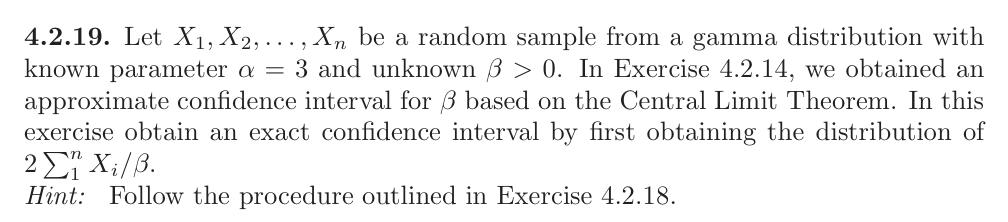
\includegraphics[width=\textwidth]{3-hw5-2025032722.png}
% \caption{}
\label{}
\end{figure}
\end{exercise}
\[
\varphi_{X_k}(t)=(1-i\beta t)^{-3}
\]
Denote $Y_n=2\sum_{k=1}^{n}X_{k}/\beta$, then
\[
\varphi_{Y_n}(t)=\mathbb{E}\left( \exp \left\{  it\cdot 2\sum_{k=1}^{n} X_k/\beta  \right\} \right)=\prod_{k=1}^{n} \varphi_{X_k}(2t/\beta)
=(1-2it)^{-3n}
\]
Thus $Y_n\sim\Gamma(3n,2)$.
\[
p_{Y_n}(x)=\frac{1}{\Gamma(3n)2^{3n}}x^{3n-1}e^{ -x/2  }\qquad 0<x<\infty
\]
Let $1-\alpha=P(Y_n<\gamma_{n,\alpha})$, then the $100\alpha\%$ confidence interval for $\beta$ is
\[
\left[ 0,\frac{2\overline{x}}{\gamma_{n,\alpha}} \right]
\]
\begin{exercise}
\begin{figure}[H]
\centering
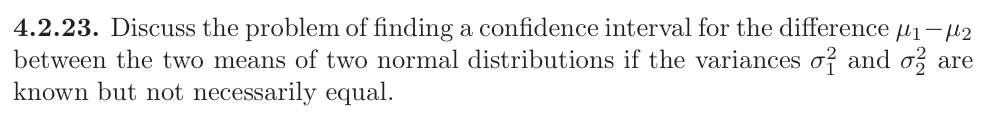
\includegraphics[width=\textwidth]{4-hw5-2025032722.png}
% \caption{}
\label{}
\end{figure}
\end{exercise}
Let $X_1,\dots,X_n$ be a random sample of $N(\mu_1,\sigma_1^2)$, $Y_1,\dots ,Y_m$ be of $N(\mu_2,\sigma_2^2)$. Then $\overline{X}_n\sim N\left( \mu_1,\frac{\sigma_1^2}{n_1} \right),\overline{Y}_n\sim N\left( \mu_2,\frac{\sigma^{2}_{2}}{n_2} \right)$. Therefore $\overline{X}_n-\overline{Y}_n\sim N\left( \mu_1-\mu_2,\frac{\sigma_1^2}{n_1}+\frac{\sigma_2^2}{n_2} \right)$. Let $\overline{x}$ and $\overline{y}$ denote the realized values of the statistics $\overline{X}$ and $\overline{Y}$. Let $z_{\alpha/2 }=\Phi ^{-1}\left( 1-\frac{\alpha}{2} \right)$ then the $(1-\alpha) 100\%$ confidence interval of $\mu_1-\mu_2$ is
\[
\left( \overline{x}-\overline{y}-z_{\alpha/2 }\left( \frac{\sigma_1^2}{n_1}+\frac{\sigma_2^2}{n_2} \right)^{1/2},\overline{x}-\overline{y}+z_{\alpha/2 }\left( \frac{\sigma_1^2}{n_1} +\frac{\sigma_2^2}{n_2}\right)^{1/2} \right)
\]
\begin{exercise}
\begin{figure}[H]
\centering
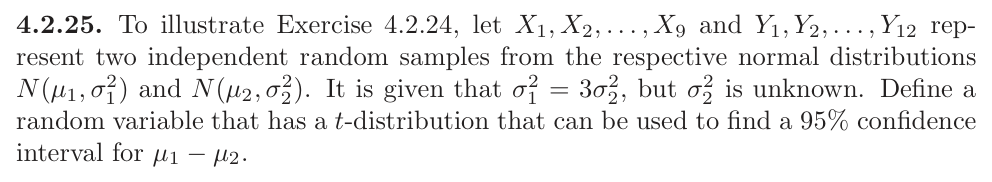
\includegraphics[width=\textwidth]{5-hw5-2025032722.png}
% \caption{}
\label{}
\end{figure}
\end{exercise}
Denote $n_1=9,n_2=12,n=n_1+n_2=21$, then
\[
\overline{X}_{n_1}\sim N\left( \mu_1,\frac{1}{n_1} \sigma_1^2 \right)\qquad \overline{Y}_{n_2}\sim N\left( \mu_2,\frac{1}{n_2} \sigma_2^2 \right)
\]
\[
\overline{X}_{n_1}-\overline{Y}_{n_2}\sim N\left( \mu_1-\mu_2,\underbrace{ \frac{1}{n_1} \sigma^{2}_{1}+\frac{1}{n_2} \sigma_2^2 }_{ =\sigma_1^2\left( \frac{1}{n_1}+\frac{1}{3n_2} \right) } \right)
\]
Thus
\[
\sqrt{ n_1 }(\overline{X}_{n_1}-\mu_1)/\sigma_1\sim N(0,1)\qquad \sqrt{ n_2 }(\overline{Y}_{n_2}-\mu_2)/\sigma_2\sim N(0,1)
\]
\[
W\coloneqq \frac{(\overline{X}_{n_1}-\overline{Y}_{n_2})-(\mu_1-\mu_2)}{\sigma_1\sqrt{ \frac{1}{n_1} +\frac{1}{3n_2}  }}\sim N(0,1)
\]
Let
\[
S_{p}^2=\frac{(n_1-1)S_1^2+3(n_2-1)S_2^2}{n-2}
\]
which is an unbiased estimator of $\sigma_1^2$. By Student's theorem,
\[
(n_1-1)S_1^2/\sigma_1^2\sim \chi^{2}(n_1-1)\qquad \underbrace{ (n_2-1)S_2^2/\sigma_2^2 }_{ =3(n_2-1)S_2^2/\sigma_1^2 }\sim \chi^{2}(n_2-1)
\]
Then
\[
(n-2)S_{p}^2/\sigma_1^2\sim \chi^{2}(n-2)
\]
And
\[
E[S_{p}^2]=\frac{1}{n-2}[(n_1-1)\sigma_1^2+3(n_2-1)\sigma_2^2]=\sigma_1^2
\]
$S_{p}^2$ is an unbiased estimator of $\sigma_1^2$. Since $S_1^2$ is independent of $\overline{X}_{n_1}$ and $S_2^2$ is independent of $\overline{Y}_{n_2}$ by Student's theorem, $S_{p}^2$ is independent of $\overline{X}_{n_1}$ and $\overline{Y}_{n_2}$. Thus
\[
T\coloneqq \frac{W}{\sqrt{ S_{p}^2/(n-2) }}=\frac{\frac{(\overline{X}_{n_1}-\overline{Y}_{n_2})-(\mu_1-\mu_2)}{\sigma_1\sqrt{ \frac{1}{n_1} +\frac{1}{3n_2}  }}}{\frac{(n_1-1)S_1^2+3(n_2-1)S_2^2}{n-2}}\sim t(n-2)
\]
Denote $t_{\alpha/2,n-2}=F_{T}^{-1}\left( 1-\frac{\alpha}{2} \right)$, $\alpha=0.05$, then the $(1-\alpha)$ confidence interval of $\mu_1-\mu_2$ is
\[
\begin{aligned}
 & \overline{X}_{n_1}-\overline{Y}_{n_2}-t_{\alpha/2,n-2}\cdot \sigma_1\cdot \sqrt{ \frac{1}{n_1} +\frac{1}{3n_2}  }\cdot\frac{(n_1-1)S_1^2+3(n_2-1)S_2^2}{n_1+n_2-2} \\
 & \leq \mu_1-\mu_2\leq \\
 &  \overline{X}_{n_1}-\overline{Y}_{n_2}+t_{\alpha/2,n-2}\cdot \sigma_1\cdot \sqrt{ \frac{1}{n_1} +\frac{1}{3n_2}  }\cdot\frac{(n_1-1)S_1^2+3(n_2-1)S_2^2}{n_1+n_2-2}
\end{aligned}
\]
We know that $t_{\alpha/2,n-2}=2.093$ thus
\[
[\overline{X}_{n_1}-\overline{Y}_{n_2}-2.093\cdot \sigma_1\cdot \frac{\sqrt{ 5 }}{6}\cdot\frac{8S_1^2+33S_2^2}{19},\overline{X}_{n_1}-\overline{Y}_{n_2}+2.093\cdot \sigma_1\cdot \frac{\sqrt{ 5 }}{6}\cdot\frac{8S_1^2+33S_2^2}{19}]
\]
i.e.
\[
[\overline{X}_{n_1}-\overline{Y}_{n_2}-14.8203\cdot\sigma_1\cdot(8S_1^2+33S_2^2),\overline{X}_{n_1}-\overline{Y}_{n_2}+14.8203\cdot\sigma_1\cdot(8S_1^2+33S_2^2)]
\]
\begin{exercise}[(a)(c)]
\begin{figure}[H]
\centering
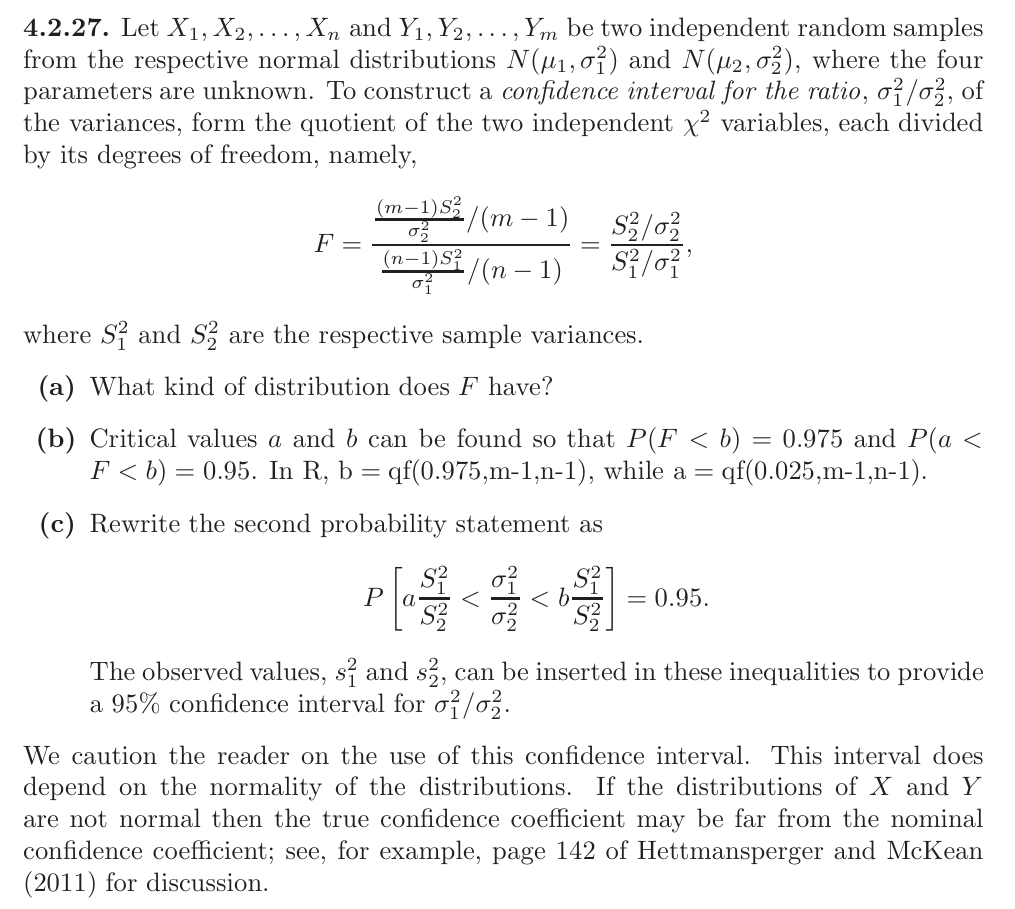
\includegraphics[width=\textwidth]{6-hw5-2025032722.png}
% \caption{}
\label{}
\end{figure}
\end{exercise}
(a)
\[
(m-1)S_2^2/\sigma_2^2\sim \chi^{2}(m-1)\qquad (n-1)S_1^2/\sigma_1^2\sim \chi^{2}(n-1)
\]
Then
\[
F=\frac{\frac{(m-1)S_2^2}{\sigma_2^2}/(m-1)}{\frac{(n-1)S_1^2}{\sigma_1^2}/(n-1)}\sim F(m-1,n-1)
\]
(c)
Trivial.

\begin{exercise}
\begin{figure}[H]
\centering
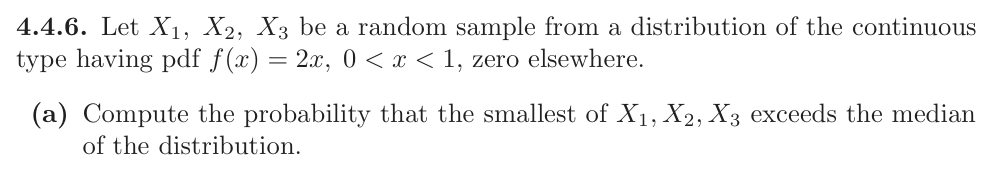
\includegraphics[width=\textwidth]{7-hw5-2025032722.png}
% \caption{}
\label{}
\end{figure}
\end{exercise}
Let $Y_1,Y_2,Y_3$ denote the 3 order statistics based on the random sample $X_1,X_2,X_3$, then the joint pdf of $Y_1,Y_2,Y_3$ is given by
\[
g(y_1,y_2,y_3)=\begin{cases}
6f(y_1)f(y_2)f(y_3) & 0<y_1<y_2<y_3<1 \\
0 & \text{elsewhere}
\end{cases}
\]
Then
\[
\begin{aligned}
\mathbb{P}\left( Y_1\geq \frac{1}{2} \right) & =\int_{1/2 }^{1} \int_{y_1}^{1} \int_{y_2}^{1} 6f(y_1)f(y_2)f(y_3) \, dy_3  \, dy_2  \, dy_1 \\
 & =\int_{1/2 }^{1} \int_{y_1}^{1} \int_{y_2}^{1} 48y_1y_2y_3  \, dy_2  \, dy_1  \\
 & =\int_{\frac{1}{2}}^{1} \int_{y_1}^{1} 24y_1y_2(1-y_2^2) \, dy_2  \, dy_1  \\
 & =\int_{\frac{1}{2}}^{1} 12y_1(1-y_1^2)-6y_1(1-y_1^{4}) \, dy_1 \\
  & =\int_{\frac{1}{2}}^{1} (6y_1-12y_1^3+6y_1^{5}) \, dy_1  \\
 & =\frac{27}{64} 
\end{aligned} 
\]
\begin{exercise}
\begin{figure}[H]
\centering
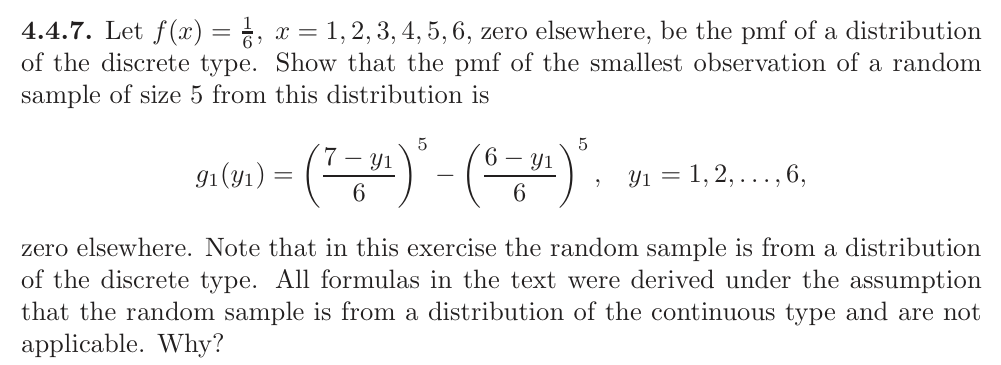
\includegraphics[width=\textwidth]{8-hw5-2025032722.png}
% \caption{}
\label{}
\end{figure}
\end{exercise}
\[
P(Y_1=1)=1-\left( \frac{5}{6} \right)^{5}
\]
\[
P(Y_1=2)=\left( \frac{5}{6} \right)^{5}-\left( \frac{4}{6} \right)^{5}
\]
\[
P(Y_1=3)=\left( \frac{4}{6} \right)^{5}-\left( \frac{3}{6} \right)^{5}
\]
\[
P(Y_1=4)=\left( \frac{3}{6} \right)^{5}-\left( \frac{2}{6} \right)^{5}
\]
\[
P(Y_1=5)=\left( \frac{2}{6} \right)^{5}-\left( \frac{1}{6} \right)^{5}
\]
\[
P(Y_1=6)=\left( \frac{1}{6} \right)^{5}-(0)^{5}
\]
That is
\[
g_1(y_1)=\left( \frac{7-y_1}{6} \right)^{5}-\left( \frac{6-y_1}{6} \right)^{5},\qquad y_1=1,2,\dots,6
\]
\begin{exercise}
\begin{figure}[H]
\centering
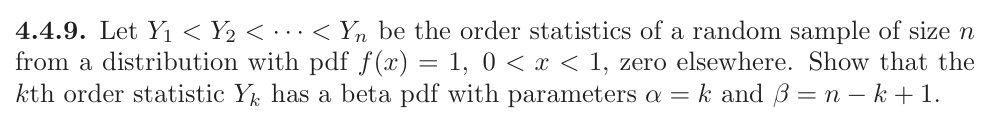
\includegraphics[width=\textwidth]{9-hw5-2025032722.png}
% \caption{}
\label{}
\end{figure}
\end{exercise}
\[
g(y_1,y_2,\dots,y_n)=n!\cdot f(y_1)\cdot\dots \cdot f(y_n)=n!,\quad 0<y_1<y_2<\dots<y_n<1
\]
Then
\[
\begin{aligned}
p_{Y_k}(y_k) & =\int_{(0,y_k)\times (y_1,y_k)\times \dots \times(y_{k-2},y_k)\times(y_k,1)\times(y_{k},y_n)\times\dots \times(y_k,y_{k+2})}^{} n! \, dy_1dy_2\dots dy_{k-1}\cdot dy_ndy_{n-1}\dots d_{k+1} \\
 & =\frac{y_k^{k-1}}{(k-1)!}\cdot\frac{(1-y_k)^{n-k}}{(n-k)!}\cdot n! \\
 & =\frac{\Gamma(n+1)}{\Gamma(k)\Gamma(n-k+1)}y_k^{k-1}(1-y_k)^{n-k+1} 
\end{aligned}
\]
\begin{exercise}
\begin{figure}[H]
\centering
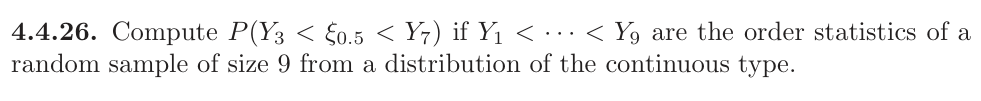
\includegraphics[width=\textwidth]{10-hw5-2025032722.png}
% \caption{}
\label{}
\end{figure}
\end{exercise}
\[
P(Y_3<\xi_{0.5}<Y_7)=\sum_{n=3}^{6} {\binom{9}{n} }0.5^{n}\cdot 0.5^{9-n}=\frac{105}{128}
\]
\begin{exercise}
\begin{figure}[H]
\centering
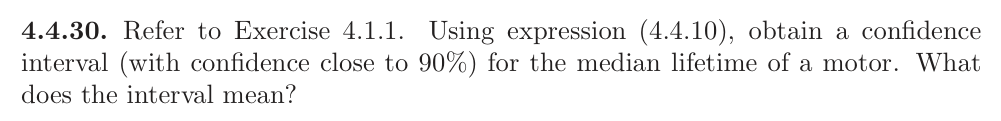
\includegraphics[width=\textwidth]{11-hw5-2025032722.png}
% \caption{}
\label{}
\end{figure}
\end{exercise}
\begin{figure}[H]
\centering
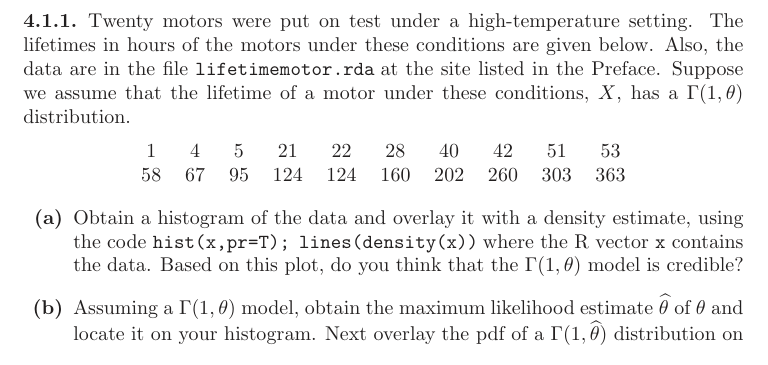
\includegraphics[width=\textwidth]{hw5-2025033022.png}
% \caption{}
\label{}
\end{figure}

For binomial distribution $B\left( 20,\frac{1}{2} \right)$, $F^{-1}(0.05)=6$ thus
\[
(y_7,y_{14})=(40,124)
\]
is a $90\%$ confidence interval for $\xi_{\frac{1}{2}}$.

The interval means that the median number has the probability $90\%$ lying the interval $(40,124)$.

\begin{exercise}
\begin{figure}[H]
\centering
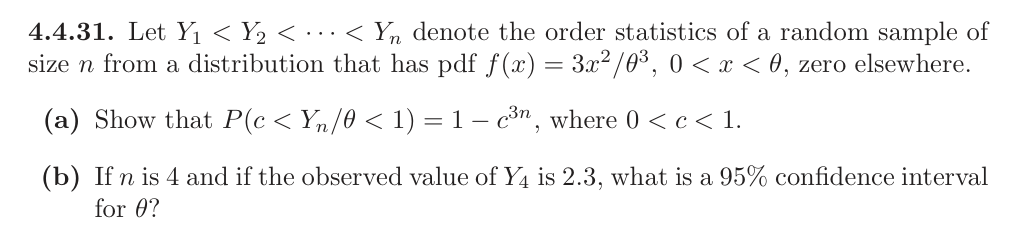
\includegraphics[width=\textwidth]{12-hw5-2025032722.png}
% \caption{}
\label{}
\end{figure}
\end{exercise}
(a)
\[
g(y_1,\dots,y_n)=n!\cdot\frac{3^{n}\cdot y_1^2\cdot \dots \cdot y_n^2}{\theta^{3n}}
\]
Then
\[
\begin{aligned}
P(c<Y_n/\theta<1) & =P(c\theta <Y_n<\theta) \\
 & =1-P(Y_n\leq c\theta) \\
 & =1-P(\max_{1\leq k\leq n}X_k\leq c\theta) \\
 & =1-\prod_{k=1}^{n} P(X_k\leq c\theta) \\
 & =1-\prod_{k=1}^{n} \int_{0}^{c\theta} \frac{3x^2}{\theta^{3}} \, dx \\
  & =1-\prod_{k=1}^{n} c^{3} \\
 & =1-c^{3n}
\end{aligned}
\]
(b)
$n=4$ and $Y_4=2.3$, then
\[
P(c<Y_4/\theta<1)=P\left( 2.3<\theta<\frac{2.3}{c} \right)=1-c^{12}
\]
Then the $95\%$ confidence interval for $\theta$ can be
\[
(2.3,2.95221)
\]